% Editable reconstruction; interpretation recorded in root.json.
% Shared standalone design for the editable figure reconstructions.
\documentclass[tikz,border=5pt,10pt]{standalone}
\usepackage[T1]{fontenc}
\usepackage[utf8]{inputenc}
\usepackage{newpxtext,newpxmath}
\usepackage[scaled=.94]{sourcesanspro}
\usepackage{pgfplots}
\pgfplotsset{compat=1.18}
\usetikzlibrary{arrows.meta,calc,positioning,decorations.pathreplacing,
  decorations.markings,patterns,matrix,shapes.geometric,fit,backgrounds,
  intersections,angles,quotes}
\definecolor{ink}{HTML}{203746}
\definecolor{accent}{HTML}{146C78}
\definecolor{muted}{HTML}{667780}
\definecolor{signalred}{HTML}{B94B44}
\color{ink}
\tikzset{>=Latex,line width=.8pt,
  every node/.style={font=\small},
  axis/.style={->,draw=muted,line width=.5pt},
  guide/.style={draw=muted,dashed,line width=.45pt},
  curve/.style={draw=accent,line width=1pt},
  marker/.style={circle,fill=accent,inner sep=1.5pt},
  labelbox/.style={fill=white,inner sep=2pt}}

\begin{document}
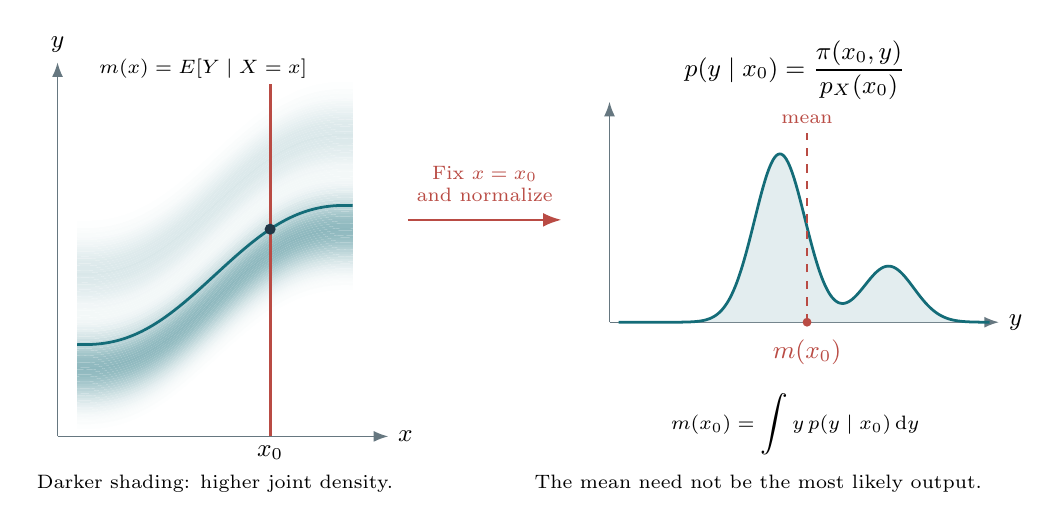
\begin{tikzpicture}[x=1cm,y=1cm]
\pgfmathdeclarefunction{mean}{1}{\pgfmathparse{.4*#1+.35*sin(85*#1)}}
% Centered but asymmetric noise: .75*(-.3)+.25*(.9)=0.
\pgfmathdeclarefunction{noise}{1}{\pgfmathparse{
 (.75*exp(-((#1+.3)/.28)^2/2)+.25*exp(-((#1-.9)/.28)^2/2))/(.28*sqrt(2*pi))}}
\pgfmathsetmacro{\conditionalmean}{mean(.7)}
\begin{scope}
\draw[axis] (-2,-2.05)--(2.2,-2.05) node[right] {$x$};
\draw[axis] (-2,-2.05)--(-2,2.7) node[above] {$y$};
% Let X be uniform on [-1.75,1.75], independent of the mixture noise.
% Joint density is noise(y-mean(x))/3.5 on that strip. The color scale is
% relative to its maximum; the finite y window is not a support claim.
\foreach \j in {0,...,89}{
 \pgfmathsetmacro{\lo}{-1.1+.03*\j}
 \pgfmathsetmacro{\hi}{\lo+.031}
 \pgfmathtruncatemacro{\shade}{min(48,45*noise(\lo+.015))}
 \fill[accent!\shade] plot[domain=-1.75:1.75,samples=70] (\x,{mean(\x)+\lo})
  --plot[domain=1.75:-1.75,samples=70] (\x,{mean(\x)+\hi})--cycle;
}
\draw[curve,domain=-1.75:1.75,samples=100] plot (\x,{mean(\x)});
\draw[signalred,line width=1pt] (.7,-2.05)--(.7,2.45);
\fill[ink] (.7,\conditionalmean) circle(2pt);
\node[below] at (.7,-2.05) {$x_0$};
\node[font=\scriptsize,fill=white,inner sep=2pt] at (-.15,2.62) {$m(x)=\mathbb E[Y\mid X=x]$};
\node[font=\scriptsize] at (0,-2.65) {Darker shading: higher joint density.};
\end{scope}
\draw[->,signalred,line width=.8pt] (2.45,.7)--(4.4,.7)
 node[midway,above=3pt,font=\scriptsize,align=center] {Fix $x=x_0$\\and normalize};
\begin{scope}[shift={(6.85,-.6)},x=1.15cm,y=2cm]
\draw[axis] (-1.6,0)--(2.7,0) node[right] {$y$};
\draw[axis] (-1.6,0)--(-1.6,1.4);
\fill[accent!12] (-1.5,0) plot[domain=-1.5:2.6,samples=220]
 (\x,{noise(\x-\conditionalmean)})--(2.6,0)--cycle;
\draw[curve,domain=-1.5:2.6,samples=220] plot (\x,{noise(\x-\conditionalmean)});
\draw[signalred,dashed] (\conditionalmean,0)--(\conditionalmean,1.2);
\fill[signalred] (\conditionalmean,0) circle(1.6pt);
\node[below=3pt,signalred] at (\conditionalmean,0) {$m(x_0)$};
\node[font=\scriptsize,signalred,above] at (\conditionalmean,1.2) {mean};
\node at (.45,1.6) {$\displaystyle p(y\mid x_0)=\frac{\pi(x_0,y)}{p_X(x_0)}$};
\node[font=\scriptsize] at (.45,-.65) {$\displaystyle m(x_0)=\int y\,p(y\mid x_0)\,\mathrm dy$};
\end{scope}
\node[font=\scriptsize] at (6.9,-2.65) {The mean need not be the most likely output.};
\end{tikzpicture}
\end{document}
